\documentclass{report}
\usepackage[utf8]{inputenc}
\usepackage{graphicx}
\usepackage{circuitikz}
\usepackage{tikz}
\usepackage{pgfplots}
\usepackage{biblatex}
\graphicspath{{}}

\title{Lab Work 02}
\author{Jose Antonio Domene Reyes}
\date{March 2018}

\begin{document}

\maketitle

\chapter{Theoretical part}
\section{Circuit calculation}
\begin{description}
In Laboratory work 1 we modeled a circuit using gEDA, ngspice and some advanced students also used QUCS. 
\end{description}

My student number is 181ADB018, therefore I used: 
\begin{equation}
    V1 = 018/10 = 1.8[V]
\end{equation}
\begin{equation}
    R1 = 1+1 = 2\Omega
\end{equation}
\begin{equation}
    R2 = 8+1 + 9\Omega
\end{equation}

As for the mathematical calculations we did two: 
\begin{equation}
    U_R_1 = \frac{R1}{R1+R2}*V1
\end{equation}
\begin{equation}
    U_R_2 = \frac{R2}{R1+R2}*V1
\end{equation}

\begin{figure}[!b]
    \centering
    \begin{tabular}{ |c|c| } 
        \hline
        V1 & 1.8 \\ 
        \hline
        R1 & 2 \\ 
        \hline
        R2 & 9 \\ 
        \hline
        U_R_1 & 0.327273 \\ 
        \hline
        U_R_2 & 1.472727 \\
        \hline
    \end{tabular}
    \caption{Values of circuit calculations}
\end{figure}

\begin{figure}[!t]
    \begin{center}
        \begin{circuitikz}
        \draw
        (0,0) to [european resistor, l=$R_1$] (6,0)
        to [european resistor, l=$R_2$] (6,-4)
        to [short, *-] (0,-4)
        to [battery1, l=$V_1$] (0,0)
        \end{circuitikz}
    \end{center}
    \caption{Circuit diagram}
\end{figure}

\begin{figure}[!b]
    \centering
    \begin{tikzpicture}
    \begin{axis}[xlabel=$R_2$, ylabel=$U_2$, xmin=0, xmax=6, ymin=0, ymax=2]
        \addplot{x/(2+x)*1.8};
    \end{axis}
    \end{tikzpicture}
    \caption{Function plot U(R2) = f(R2)}
\end{figure}

\chapter{Practical part}
\section{Work with gEDA programs}
\subsection{Work with gschem}
The next image is a screenshot of the circuit gschem produced.
\begin{figure}[!b]
    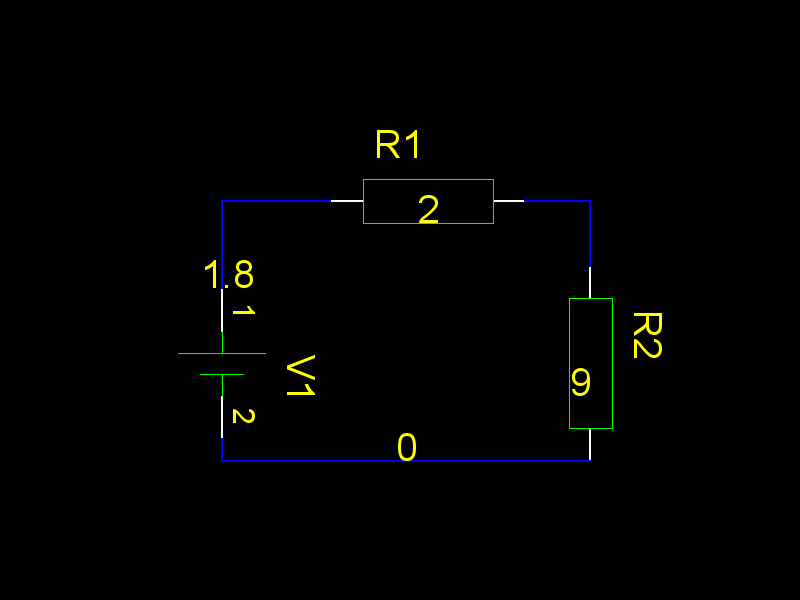
\includegraphics[scale=0.4]{circuit.png}
    \caption{Image of circuit.png}
\end{figure}
\subsection{Work with gnetlist}
%%01.net file contents
\begin{verbatim}
    * Spice netlister for gnetlist
    V1 2 0 1.8
    R1 2 1 2
    R2 1 0 9
    .END
\end{verbatim}

\subsection{Work with ngspice}
\begin{figure}[!b]
    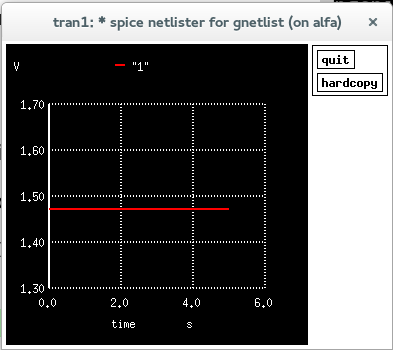
\includegraphics[scale=1]{11.png}
    \caption{Image of 11.png, first plot}
\bigbreak
\end{figure}
\hskip 5pt
\begin{figure}[!t]
    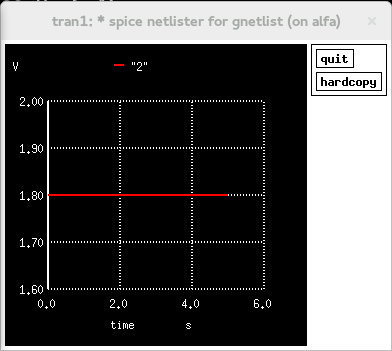
\includegraphics[scale=1]{12.png}
    \caption{Image of 12.png, second plot}
\end{figure}

\section{Work with QUCS programs}
I am not advanced enough to work with QUCS. I did not do this part in P01.

\begin{thebibliography}{9}
\bibitem{latexcompanion} 
Michel Goossens, Frank Mittelbach, and Alexander Samarin. 
\textit{The \LaTeX\ Companion}. 
Addison-Wesley, Reading, Massachusetts, 1993.
 
\bibitem{einstein} 
Albert Einstein. 
\textit{Zur Elektrodynamik bewegter K{\"o}rper}. (German) 
[\textit{On the electrodynamics of moving bodies}]. 
Annalen der Physik, 322(10):891–921, 1905.
 
\bibitem{knuthwebsite} 
Knuth: Computers and Typesetting,
\\\texttt{http://www-cs-faculty.stanford.edu/\~{}uno/abcde.html}
\end{thebibliography}



\end{document}
